France has enjoyed a long and storied history as a world leader in culture, food,
literature, film, and revolutions. Over its history, the average life expectancy of people in France
has changed notably. The time series object described below contains the annual average life
expectancy in France (measured in years lived), measured during the years 1816 to 2019. The
data is in the file FLE.txt. \\

\noindent Analyze the data in the time series and write a report addressing the following:

\begin{enumerate}[label=(\alph*)]
    \item What trend model(s) best capture the trends in French life expectancy over time?
    \item Are there any noticeable patterns, or observations apparent in the series? Can you tell from
your plot what could be the causes of your observations?
    \item Regardless of what you observe, suppose you apply some transformation to the data, how
does the new data looks like? Any changes in trend?
    \item For the various models you tried, assess the fit of the models using any tools at your disposal. Perform any necessary test to make sure sure your model is appropriate. Write down the equation of your final model. Are any transformations of the data necessary? Perform all diagnostics tests.
\end{enumerate}

\noindent Now conclude with brief summary: How the life expectancy changes over time, both long-term
over the observed period of years, and in terms of patterns of year-to-year variation. Add any
necessary graphs, tests and/or confidence interval etc...

\subsection{R Code}
\lstinputlisting[language=R]{Codes/Midterm_2_P4.R}
\subsection{Results}
\begin{enumerate}[label=(\alph*)]
    \item \begin{minipage}[!h]{\linewidth}
        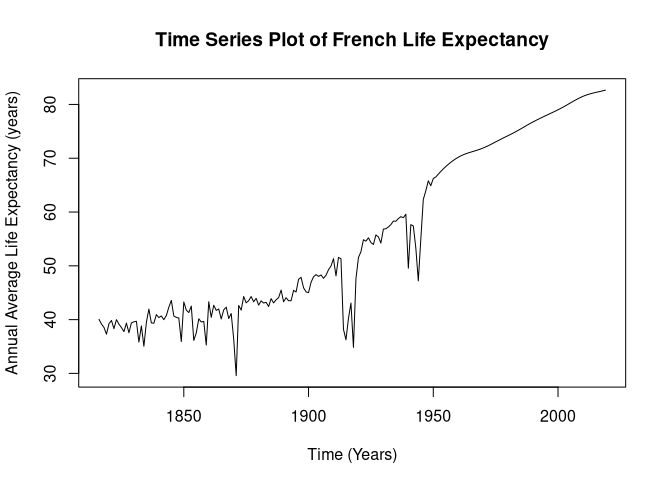
\includegraphics[width=0.9\linewidth]{Images/P4/FLE_Plot.png}
        \captionof{figure}{Time series plot of the French life expectancy data.}
        \label{fig:fle_plot}
    \end{minipage}

From Fig \ref{fig:fle_plot} it can be said that a quadratic trend is suitable for this dataset. The model summary is shown here.
\small\begin{block}
Call:
lm(formula = fle.data ~ time(fle.data) + I(time(fle.data)^2))

Residuals:
     Min       1Q   Median       3Q      Max 
-17.2140  -1.3665   0.4999   1.8464   5.6716 

Coefficients:
                      Estimate Std. Error t value Pr(>|t|)    
(Intercept)          3.499e+03  3.042e+02   11.50   <2e-16 ***
time(fle.data)      -3.849e+00  3.175e-01  -12.12   <2e-16 ***
I(time(fle.data)^2)  1.069e-03  8.279e-05   12.92   <2e-16 ***
---
Signif. codes:  0 ‘***’ 0.001 ‘**’ 0.01 ‘*’ 0.05 ‘.’ 0.1 ‘ ’ 1

Residual standard error: 3.668 on 201 degrees of freedom
Multiple R-squared:  0.946,	Adjusted R-squared:  0.9455 
F-statistic:  1762 on 2 and 201 DF,  p-value: < 2.2e-16
\end{block}
\normalsize Here, we observe that the F-statistic and the residual standard are quite high. Moreover, the augmented Dickey-Fuller stationarity test (Dickey-Fuller = -2.9107, Lag order = 5, p-value = 0.1945) confirms that the original data is not stationary. However, by only visually observing the original data (Fig \ref{fig:fle_plot}), we can say that the quadratic fit (Fig \ref{fig:qfit_fle}) is the best trend for this dataset.
\begin{figure}[!htb]
    \centering
    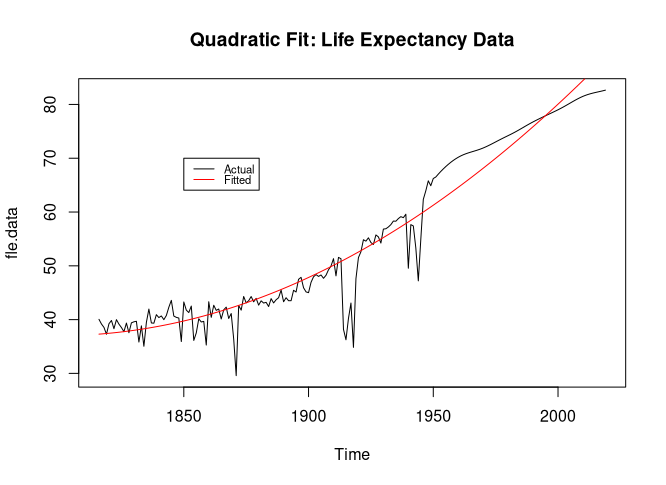
\includegraphics[width=0.9\linewidth]{Images/P4/QFit_FLE.png}
    \caption[Quadratic fit over the original French life expectancy data.]{Quadratic fit over the original French life expectancy data. The fit performs poorly from 1950 onward as we observe a linear trend from 1950-2019.}
    \label{fig:qfit_fle}
\end{figure}
\item The fluctuations in the dataset are mostly present before 1950. The increase in the life expectancy values between 1816-1850 could be attributed to the advancements in medicine. However, the sharp drops in the values, particularly during mid 1915-1920 and mid 1940s could be caused by the two world wars. Interestingly, the life expectancy increases post 1950 which could be primarily attributed to the invention of modern healthcare and economic growth.
\item \begin{minipage}[!h]{\linewidth}
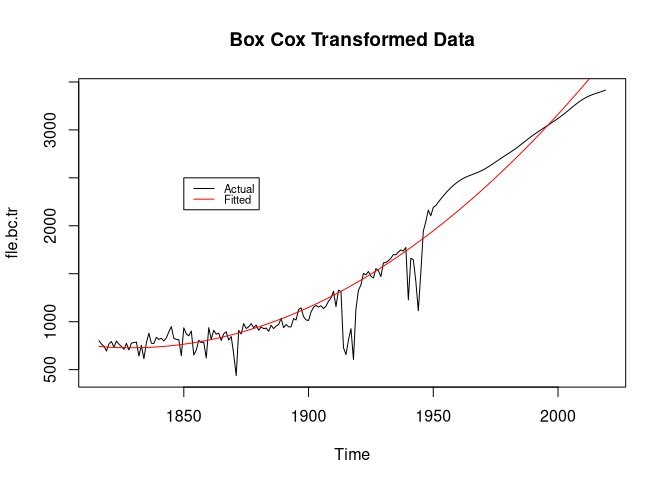
\includegraphics[width=\linewidth]{Images/P4/FLE_BC.png}
\captionof{figure}[Transformed FLE Data using Box Cox method.]{Transformed FLE Data using Box Cox method. Here, this transformation is obtained by auto-setting $\lambda \approx 1.99$. The quadratic trend still remains.}
\label{fig:qfit_bc_fle}
\end{minipage}

The model fit summary for this transformed dataset is given here.
\small\begin{block}
Call:
lm(formula = fle.bc.tr ~ time(fle.bc.tr) + I(time(fle.bc.tr)^2))

Residuals:
    Min      1Q  Median      3Q     Max 
-782.46  -70.39   23.94   83.28  305.68 

Coefficients:
                       Estimate Std. Error t value Pr(>|t|)    
(Intercept)           2.787e+05  1.494e+04   18.66   <2e-16 ***
time(fle.bc.tr)      -3.040e+02  1.559e+01  -19.50   <2e-16 ***
I(time(fle.bc.tr)^2)  8.311e-02  4.064e-03   20.45   <2e-16 ***
---
Signif. codes:  0 ‘***’ 0.001 ‘**’ 0.01 ‘*’ 0.05 ‘.’ 0.1 ‘ ’ 1

Residual standard error: 180.1 on 201 degrees of freedom
Multiple R-squared:  0.9625,	Adjusted R-squared:  0.9621 
F-statistic:  2579 on 2 and 201 DF,  p-value: < 2.2e-16
\end{block}
\normalsize
\item The residual diagnostics for the quadratic model are shown in Fig \ref{fig:res_qfit_fle}.
\begin{figure}[!htb]
    \centering
    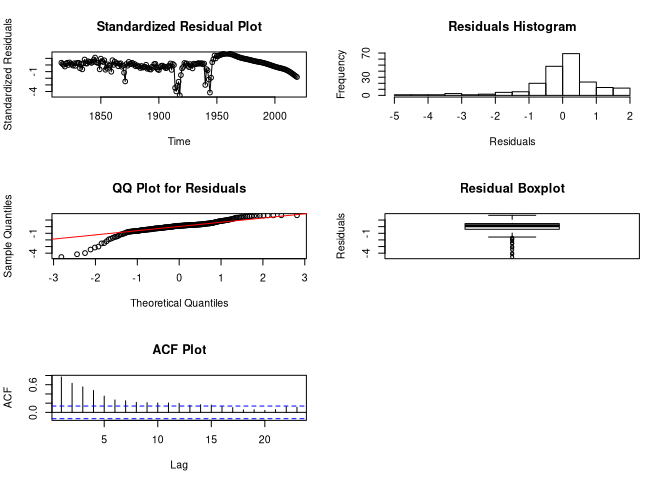
\includegraphics[width=\linewidth]{Images/P4/Residual_QFit.png}
    \caption[Residual diagnostics for the quadratic model.]{Residual diagnostics for the quadratic model. Here, we observe that this model fits poorly as the residuals follow a non-normal distribution.}
    \label{fig:res_qfit_fle}
\end{figure}
We further verify the non-normality of the residuals using the Shapiro-Wilk and Exact Runs tests.
\small\begin{block}
Quadratic Model

Shapiro-Wilk normality test
W = 0.88032, p-value = 1.21e-11

Exact runs test
Runs = 46, p-value = 3.374e-16
alternative hypothesis: two.sided
\end{block}
\normalsize Next, we detrend the transformed dataset (Fig \ref{fig:detrend_fle}) using two differences because of the quadratic trend (i.e. the transformed dataset is not stationary). Since no seasonality is present, we set lag=1.
\begin{figure}[!htb]
    \centering
    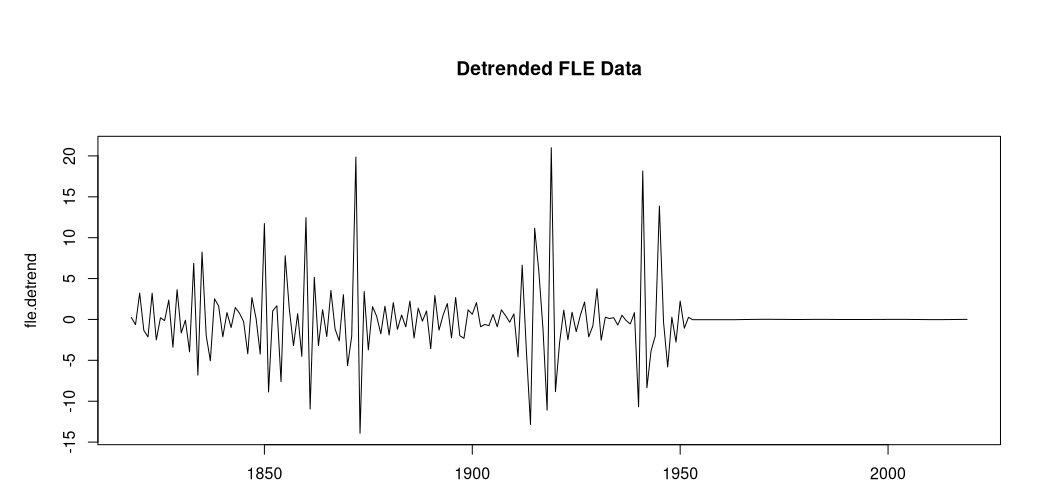
\includegraphics[width=\linewidth]{Images/P4/Detrend_FLE.png}
    \caption[Plot of the detrended FLE data.]{Plot of the detrended FLE data. This shows that we have achieved stationarity and can now proceed with various ARIMA modeling. We also verify this using the augmented Dickey-Fuller test (Dickey-Fuller = -10.009, Lag order = 5, p-value = 0.01) where we accept the alternative hypothesis of stationarity.}
    \label{fig:detrend_fle}
\end{figure}
Once the detrending is done, we check the ACF, PACF, EACF, and the ARMA subset plots as given in Fig. \ref{fig:acf_fle}.

\begin{figure}[!htb]
    \centering
    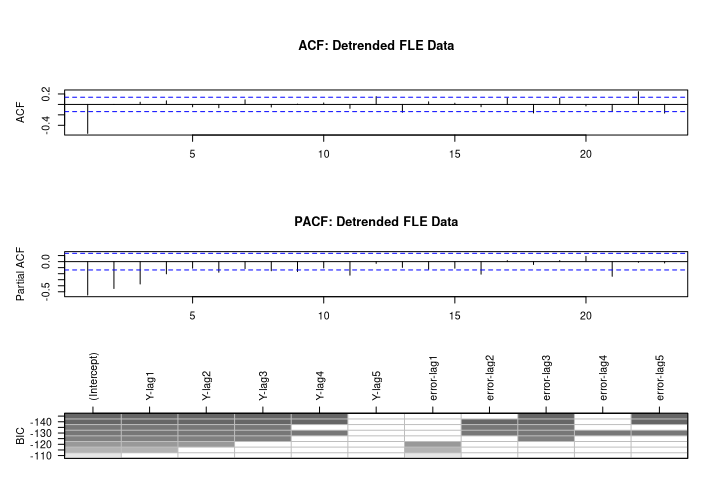
\includegraphics[width=\linewidth]{Images/P4/ACF_Plots_FLE.png}
    \caption[ACF, PACF, and ARMA subset plots of the detrended FLE data]{ACF, PACF, and ARMA subset plots of the detrended FLE data. From these we can say that ARMA(p, q) is a suitable model.}
    \label{fig:acf_fle}
\end{figure}
\small\begin{block}
> eacf(fle.detrend)

AR/MA
  0 1 2 3 4 5 6 7 8 9 10 11 12 13
0 x o o o o o o o o o o  x  x  o 
1 x o o o o o o o o o o  o  o  o 
2 x x o o o o o o o o o  o  o  o 
3 x o x o o o o o o o o  o  o  o 
4 x o x x x o o o o o o  o  o  o 
5 x x o o x o o o o o o  o  o  o 
6 x x x o o o x o o o o  o  o  o 
7 x x x o o o o x o o o  o  o  o
\end{block}
\normalsize Initially, we consider ARMA(1, 1) model or ARIMA(1, 0, 1). The model fit summary is given here.
\small\begin{block}
>arima(x = fle.detrend, order = c(1, 0, 1))

Coefficients:
          ar1     ma1  intercept
      -0.2498  -1.000     0.0017
s.e.   0.0680   0.013     0.0025

sigma^2 estimated as 6.765:  log likelihood = -482.63,  aic = 971.26
\end{block}
\normalsize We also perform the residual diagnostics (Figures \ref{fig:tsdiag_fle_arma_11} and \ref{fig:res_fle_arma_11})and apply the normality checks.
\begin{figure}[!htb]
    \centering
    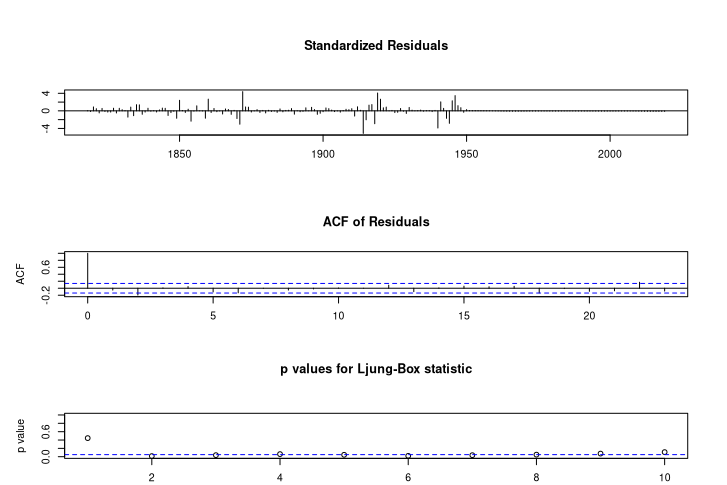
\includegraphics[width=\linewidth]{Images/P4/TSDiag_ARMA_11.png}
    \caption[Residual diagnostics for the ARMA(1, 1) model for the FLE data.]{Residual diagnostics for the ARMA(1, 1) model for the FLE data.}
    \label{fig:tsdiag_fle_arma_11}
\end{figure}
\begin{figure}[!htb]
    \centering
    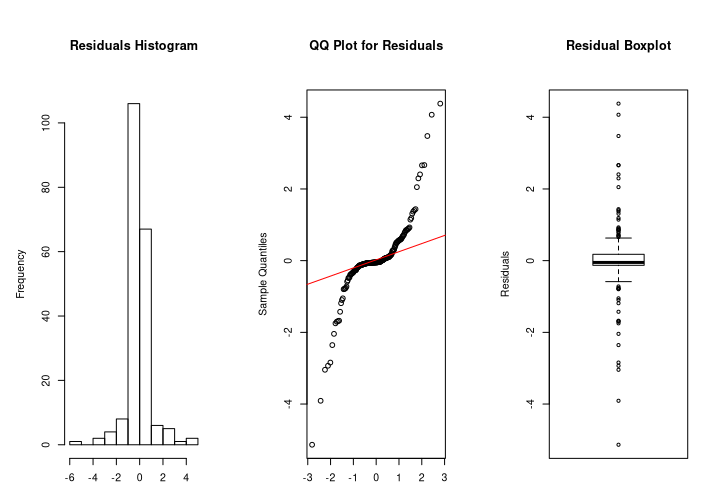
\includegraphics[width=\linewidth]{Images/P4/Residuals_FLE_ARMA_11.png}
    \caption[Residual plots for the ARMA(1, 1) model for the FLE data.]{Residual plots for the ARMA(1, 1) model for the FLE data.}
    \label{fig:res_fle_arma_11}
\end{figure}
The residual diagnostics show that the ARMA(1, 1) residuals do not closely follow a normal distribution. This is further confirmed by the Shapiro-Wilk and Runs tests.
\small\begin{block}
ARMA(1, 1) for the detrended FLE data

Shapiro-Wilk normality test
W = 0.76725, p-value < 2.2e-16

Exact runs test
Runs = 86, p-value = 0.02855
alternative hypothesis: two.sided

> AIC(model)
[1] 973.2626
> BIC(model)
[1] 986.4957
\end{block}
\normalsize Next, we try with ARMA(1, 2) to see if we have a better fit.
\small\begin{block}
Call:
arima(x = fle.detrend, order = c(1, 0, 2))

Coefficients:
         ar1      ma1     ma2  intercept
      0.5658  -1.8831  0.8831     0.0017
s.e.  0.0946   0.0600  0.0594     0.0009

sigma^2 estimated as 6.266:  log likelihood = -476.12,  aic = 960.25
\end{block}
\normalsize The residual diagnostics (Figures \ref{fig:tsdiag_fle_arma_12} and \ref{fig:res_fle_arma_12}) and normality checks are carried out like before.
\begin{figure}[!htb]
    \centering
    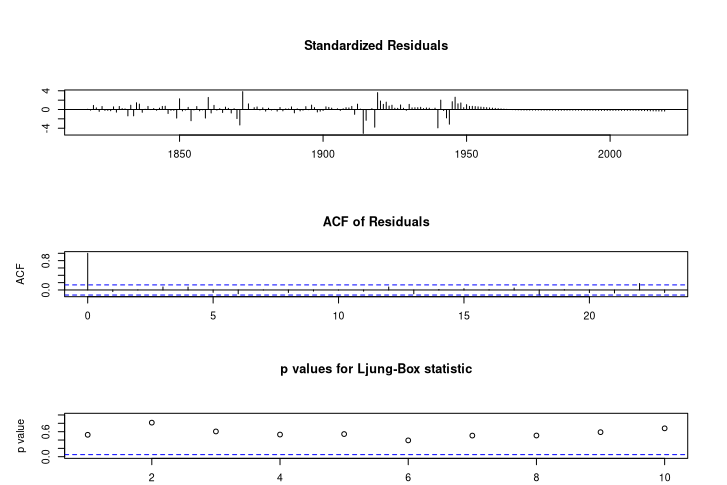
\includegraphics[width=\linewidth]{Images/P4/TSDiag_FLE_ARMA_12.png}
    \caption[Residual diagnostics for the ARMA(1, 2) model for the FLE data.]{Residual diagnostics for the ARMA(1, 2) model for the FLE data.}
    \label{fig:tsdiag_fle_arma_12}
\end{figure}
\begin{figure}[!htb]
    \centering
    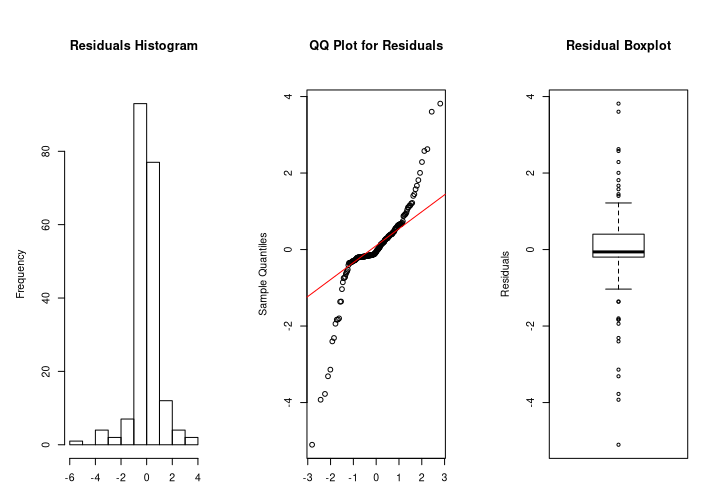
\includegraphics[width=\linewidth]{Images/P4/Residuals_FLE_ARMA_12.png}
    \caption[Residual plots for the ARMA(1, 2) model for the FLE data.]{Residual plots for the ARMA(1, 2) model for the FLE data.}
    \label{fig:res_fle_arma_12}
\end{figure}
The residual diagnostics show that the ARMA(1, 1) residuals do not closely follow a normal distribution. This is further confirmed by the Shapiro-Wilk and Runs tests.
\small\begin{block}
ARMA(1, 2) for the detrended FLE data

Shapiro-Wilk normality test
W = 0.81151, p-value = 6.773e-15

Exact runs test
Runs = 66, p-value = 4.192e-07
alternative hypothesis: two.sided

> AIC(model)
[1] 962.246
> BIC(model)
[1] 978.7874
\end{block}
\normalsize From these we can conclude that ARMA(1, 1) is preferred model. However, to obtain a better fit, we use the auto.arima function and check the effect of transformation. The model summary including the AIC and BIC values and the confidence intervals of the parameters are given here.
\small\begin{block}
> fle.auto.arima = auto.arima(fle.detrend)
> fle.auto.arima
Series: fle.detrend 
ARIMA(1,0,3) with zero mean 

Coefficients:
         ar1      ma1     ma2      ma3
      0.7382  -2.0855  1.2361  -0.1467
s.e.  0.0960   0.1212  0.2218   0.1026

sigma^2 estimated as 6.436:  log likelihood=-475.51
AIC=961.01   AICc=961.32   BIC=977.55

> fle.bc.auto.arima = auto.arima(fle.detrend, lambda="auto")
> fle.bc.auto.arima
Series: fle.detrend 
ARIMA(1,0,2) with non-zero mean 
Box Cox transformation: lambda= 0.7566293 

Coefficients:
         ar1      ma1     ma2     mean
      0.5021  -1.6531  0.7389  -1.3864
s.e.  0.2453   0.1990  0.1701   0.0253

sigma^2 estimated as 4.409:  log likelihood=-435.52
AIC=881.04   AICc=881.34   BIC=897.58

> confint(fle.bc.auto.arima)
                2.5 %     97.5 %
ar1        0.02135014  0.9827585
ma1       -2.04318152 -1.2630966
ma2        0.40548839  1.0722244
intercept -1.43600896 -1.3367935
\end{block}
\normalsize Here, we see that the transformed dataset has lower AIC and BIC values along with lesser parameters wherein the confidence intervals do not contain zero. Therefore, data transformation is required.

So from the above analyses, the final model chosen is the ARIMA(1, 0, 2) model where BoxCox transformation ($\lambda \approx 0.75$) is used. The model equation is given by Eq. \eqref{eq:final_model}.
\begin{equation}
    Z_t = -1.3864 + 0.5021Z_{t-1} + 1.6531\varepsilon_{t-1} -0.7389\varepsilon_{t-2} + \varepsilon_t
    \label{eq:final_model}
\end{equation}
 where $\varepsilon \sim \mathcal{N}(0, 4.409)$ and $Z_t = $ BoxCox($X_t$, $\lambda$), $\lambda \approx 0.75$, $t = \{1, 2, 3, \dots\}$, and $X_t$ being the original FLE data.
\end{enumerate}

\noindent If the entire duration of the time series is considered, then the life expectancy has greatly varied before 1950 but there is an overall increase in the life expectancy. From 1950 onward, the life expectancy is mostly the same. 

\noindent When individual years are taken into account, then the sharp increments and decrements in the values can be attributed to the improved healthcare systems and degrading economy or wars respectively.